

%************************************************
\chapter{Implementation and evaluation}
\label{cap:implementation}
%************************************************

The previous chapters presented the Conceptual Model and the Use-cases of a
framework for web-based human and machine computation. In this chapter are
presented the actual implementation of the framework and the use-cases.
The framework implementation is dived in two parts: the Configurator, managed by
the Crowdsearcher (see \autoref{sec:bg:crowd:cs}), and the Execution Layer
implemented in NodeJS.
The use-cases are built in \js{} and  the Execution Layer and leverages on
the \ac{HTML}5 features described in \autoref{sec:bg:web:html5}.

\section{Architecture}
\label{sec:implementation:arch}
In this section we present the architecture of our framework, whose implementation
is divided in two parts. The reference model in \autoref{fig:architecture} has
been customized to meet our needs in terms of flexibility and pluggability.
As one can see in \autoref{fig:architecture2} the Central Hub has been splitted
into two separated components: the \emph{Configurator} and the \emph{Execution Layer}.
The \emph{Configurator} is in charge of managing the Tasks lifecycle. It is used
to create and configure the Tasks.
The \emph{Execution Layer} is used to configure the actual implementations for
each \utask{}.

\begin{figure}[htb]
    \centering
    
\includegraphics[width=\columnwidth]{Architecture2}
    \caption{Specialized architecture.}
    \label{fig:architecture2}
\end{figure}

\subsection{Configurator}\label{sec:configurator}
The \textbf{Configurator} is in charge of managing the Tasks lifecycle
from the abstract definition to the results aggregation. This component must
implement the metamodel described in \ref{data:model} to describe the Tasks and
must handle correctly the the hooks defined in \ref{sec:model:strategies}. This
component must have a set of API for the Task management.
The main functionality offered by the \emph{Configurator} are:
\begin{itemize}
    \item Allow the \textbf{creation} of a Task, also at abstract level, using
    either the API or the built-in UI.

    \item Allow a \emph{Performer} to \textbf{execute} the Task using a standard
    non configurable UI, provided as-is for each Task type.

    \item Allow to \textbf{request information} about a Task, the information
    that can be requested includes:
    \begin{itemize}
        \item Retrieve the list of \utask{} associated with a given Task

        \item Post the result of the execution of a given \utask{}

        \item Notify about the completion of a Task or \utask{}
    \end{itemize}
\end{itemize}

\noindent For implementing this component we adopted the
\emph{CrowdSearcher} framework.
As described in \ref{sec:bg:crowd:cs} this framework natively embodies most of
the functionality described previously. The \emph{CrowdSearcher} supports most
of the operations required by our framework natively. The \emph{Task creation}
and the \emph{Task planning} built-in implementations are now described to
better understand how the framework works.

\subsubsection{Task creation}
The task creation if performed by the \emph{Configurator} either by using its
web-interface or via API calls. The creation of a Work/Task can be performed with
three methods: using a JSON file, via API calls or using a step-by-step "manual" procedure.
Using a JSON file, user can supply file containing all the required information like
the data definition and the data instances.
Otherwise the user create the new Task following a step-by-step procedure bundled
with the \emph{Configurator}. As shown in \autoref{fig:task-creation} the manual Task
creation involves the definition of a \textbf{Schema} for the data with all the
related Fields. Once the Schema has been defined the user can supply the data
instances to the Task.

\begin{figure}[htb]
    \centering
    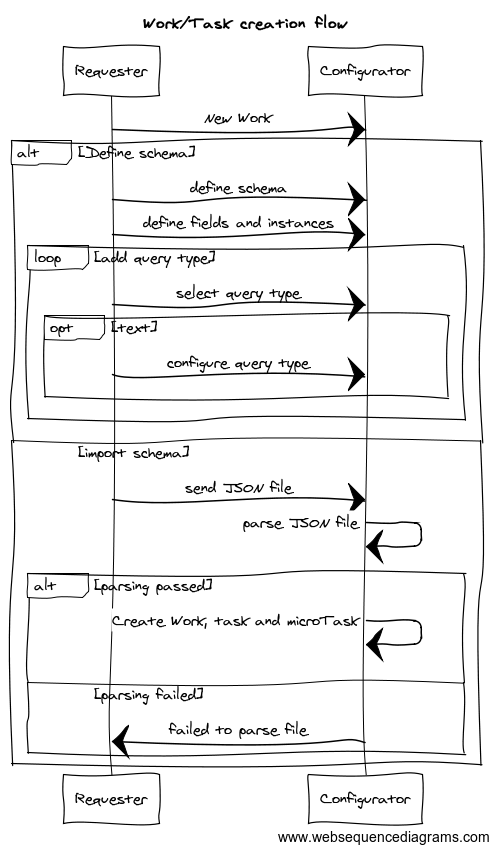
\includegraphics[width=0.65\columnwidth]{task-creation}
    \caption{Work/Task creation flow.}
    \label{fig:task-creation}
\end{figure}



\subsubsection{Task planning}
\begin{figure}[htb]
    \centering
    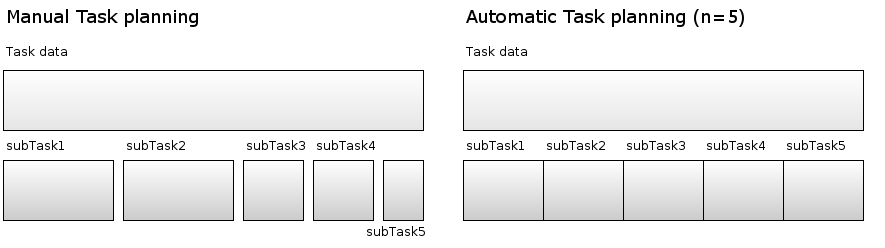
\includegraphics[width=\columnwidth]{planning}
    \caption{Manual Task planning vs Automatic Task planning.}
    \label{fig:auto-manual-planning}
\end{figure}
The planning of a Task involves the creation of \utask{} with the associated data.
The assignment can be performed either automatically or manually.
The automatic plan assignment uses a simple subdivision based on the
number of instances to assign to each \utask{} (see \autoref{auto-manual-planning}).

As depicted in \autoref{fig:task-planning} manual planning involves the
\emph{Requester} interaction in order to create each \textbf{\utask{}}.
After the creation of the \utask{} the user have to select the instances belonging
to this \utask{}. Eventually the user is able to select and, if needed,
configure the type of the \utask{}. The configurable types must be a subset of
the parent Task types.
\begin{figure}[htb]
    \centering
    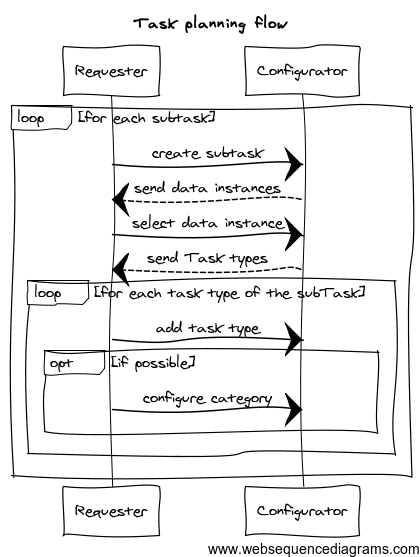
\includegraphics[width=0.65\columnwidth]{task-planning}
    \caption{Task planning flow.}
    \label{fig:task-planning}
\end{figure}










\subsection{Execution layer}\label{sec:exec-layer}
The \emph{Execution Layer} is in charge of managing the \utask{} implementations.
As described in \ref{data:task}, each Task belongs to a macro-type (i.e.
classify, like, comment, etc), and each macro-type  has its own built-in
implementation. The \emph{Execution Layer} give an easy overriding method to
replace the built-in UI with a custom one.
Using the \emph{Execution Layer} a user is able to upload the executable resources
(e.g. HTML, \js{}) that will be used as the new interface.
This custom implementations can be defined hierarchically for each Task
and \utask{}. So we can supply custom code for the whole Task or
for each \utask{}. Using this system we have the ability to tweak single
Tasks without harming the others. The layer provides a fallback
system for finding the most suitable code for each \utask{}.

The \textbf{Execution layer} offer the following functionalities:
\begin{itemize}
    \item Allow a \emph{Requester} to configure the implementations associated to
    a Task and/or a \utask{}. The implementations are configured specifying the
    target platform (mobile, desktop, tablet, ...) and the executable resources
    used by the implementation (i.e. HTML, CSS and JS files). Which implementation
    to use is configured later in the \emph{Planning} step.

    \item Create a layer of abstraction between the implementation and the
    Configurator, creating a sandboxed environment where the implementation can
    run and communicate with the Configurator.

    \item Allow the \emph{Performer} to execute a specific \utask{} implementation.
\end{itemize}

\noindent The \emph{Execution Layer} has been developed using \citetitle{node}.
\citetitle{node} is a platform built on Chrome's \js{} runtime for easily building fast,
scalable network applications. \citetitle{node} uses an event-driven, non-blocking I/O model
that makes it lightweight and efficient, perfect for data-intensive real-time
applications that run across distributed devices. Due to the great hype
around \citetitle{node} and the ease of developing new libraries, there are
thousands of these being developed and made available via the built-in
package manager \code{npm}.\\

The implementation of the \emph{Execution Layer} is subdivided into two parts:
the \emph{Server Backend} and the \emph{\utask{}s Wrapper}.

\paragraph{Server Backend} is a node REST web-server implemented using
\citetitle{express}. This server provides an web interface for managing the
implementations of Tasks and \utask{}s. This interface allows a user to upload
custom code (e.g. HTML, JS, CSS) for the selected Task (or \utask{}).
The Server interacts with the \emph{Configurator} to gather information on
a Task composition and type.

\paragraph{\utask{}s Wrapper} exposes a wrapper class that can be used by the
\utask{}s implementations to communicate with the \emph{Server Backend}. The
envelops the \utask{} and supply useful methods to retrieve Task configurations,
gather the associated data and post the results \emph{Configurator}.\\





\subsection{Task storage \& task runtime storage}
These are the storage areas where we put all the data associated with the Tasks
and the \utask{}s implementations. We used two separated storage area to physically
separate the runtime data from the abstract configuration of the Task.

The \emph{Task Storage} is handled by the \emph{Configurator}, meanwhile the
\emph{Task Runtime Storage} is managed by the \emph{Execution Layer}.\\



\subsection{Performer \& Performer Client}
The \emph{Performer client} represents the platforms (like desktop or mobile) on
which a \emph{Performer} executes a Task implementation. The \emph{Performer
client} make use of the \emph{Execution layer} API to retrieve the correct
implementation, communicate the status during the execution of a \utask{} and
post the result of the execution. The \emph{Performer} is the actual user that
is using the \emph{client}.






















\section{Use cases}
\label{sec:implementation:use-cases}

The previous section presented the implementation of the framework described in
this thesis. Now we describe the implementation of the three use-cases described
in chapter \ref{cap:cases}: Automatic, Human and Hybrid.

\subsection{Automatic}
% TODO ???
If a Task typically performed on high-end machines can be offloaded to web
clients we are able to use the browser as a node for \acl{DC}.

As described in \ref{sec:cases:automatic} in this
scenario we are implementing the \acf{SIFT} algorithm. This algorithm
was chosen due to its high computational requirements.

We made some preliminary tests to check if we can implement this algorithm using
pure \js{} code but we stumbled across the problems described in
\nameref{html5:workers}. Due to this limitation we opted to implement the
code using \ac{WebCL} (see \ref{sec:bg:web:webcl}). With this framework we can
leverage on the \ac{GPGPU} power to perform the computations and unburden the
\js{} engine.\\ 

In order to build a working example of the algorithm we started with the creation
of an \emph{Abstraction Layer} over the \ac{WebCL} raw implementation. Then we created
a small \emph{MultiMedia Library} able to interact with the \emph{Abstraction
Layer} for performing the CPU intensive operations. Eventually we implemented the
\ac{SIFT} algorithm within the \emph{MultiMedia Library}.

\paragraph{The abstraction layer} allow an easy communication with the \ac{WebCL}
framework. As described in \ref{sec:bg:web:webcl}, for running a OpenCL/WebCL
program a few step must be performed. Here is the list:
\begin{enumerate}
    \item Query host for \ac{OpenCL} devices.
    \item Create a context to associate \ac{OpenCL} devices.
    \item Create programs for execution on one or more associated devices.
    \item From the programs, select kernels to execute.
    \item Create memory objects accessible from the host and/or the device.
    \item Copy memory data to the device as needed.
    \item Provide kernels to the command queue for execution.
    \item Copy results from the device to the host.
\end{enumerate}
\noindent Our \emph{Abstraction Layer} allow to define all the I/O parameters
first and then run the selected \code{kernel} function on top of these. This abstraction
allowed us to easily interact with \ac{WebCL} without performing all the previous
steps each time we need to execute a \code{kernel} function.


\paragraph{The MultiMedia library} is a set of image operations implemented using
both \js{} and the OpenCL kernel language. With this library we provided a minimal
set of common operations (e.g. convolve, blur, resize, etc.) useful for the
implementation of the \ac{SIFT} algorithm.\\

\paragraph{The algorithm} has been implemented using the methods of the
\emph{MultiMedia library}. The algorithm has been implemented step-by-step
as described in \ref{case:auto:sift}. For each step the intermediate result
is stored and the step itself is timed to find bottlenecks. In
\autoref{fig:Automatic2} and \autoref{fig:Automatic3} are presented the
intermediate results obtained during the process and the final result.
\begin{figure}[htb]
    \centering
    
\includegraphics[width=\columnwidth]{Automatic2}
    \caption{Intermediate results of the algorithm.}
    \label{fig:Automatic2}
\end{figure}

\begin{figure}[htb]
    \centering
    
\includegraphics[width=\columnwidth]{Automatic3}
    \caption{\acs{SIFT} result comparison with the reference data.}
    \label{fig:Automatic3}
\end{figure}





\subsubsection{Benchmark/Metric}
Since the purpose of this use-case is the feasibility of high load computation
on the user browser, the implementation of the algorithm has not been optimized.
Then the performance of this implementation are not comparable to the existing
C/C+ implementation+, but we can leverage on the parallelism of the whole
framework to obtain an higher throughput. In our test cases we obtained the
results presented in \autoref{tab:auto-data}.
\begin{table}[htb]
    \caption{\acs{SIFT} algorithm time performances on the Web.}
    \label{tab:auto-data}
    \centering
    \begin{tabular}{c|c|c|c}
        \textbf{Image size} & \textbf{ScaleSpace + Dog} & \textbf{Keypoints
        detection} & \textbf{Total time}\\
        \hline
        1024x683 & \textasciitilde{}4300 ms & \textasciitilde{}1100 ms & \textasciitilde{}5400 ms\\
        \hline
        800x534 & \textasciitilde{}2600 ms & \textasciitilde{}700 ms & \textasciitilde{}3400 ms\\
        \hline
        600x401 & \textasciitilde{}1500 ms & \textasciitilde{}360 ms & \textasciitilde{}1900 ms\\
        \hline
        400x360 & \textasciitilde{}1130 ms & \textasciitilde{}310 ms & \textasciitilde{}1500 ms\\
        \hline
    \end{tabular}
\end{table}

















\subsection{Human}
In this scenario we implemented a \acf{WSD} problem (see \ref{sec:cases:human}).
To test our framework we built an \acl{HC} application like AIDA. The purpose of
this application is to let the user disambiguate the words in a piece of text.
This application allowed us to test also the connection capabilities of our
framework. Since the Task we implemented need to communicate to external servers
to gather the information on a word.

\begin{figure}[htb]
    \centering
    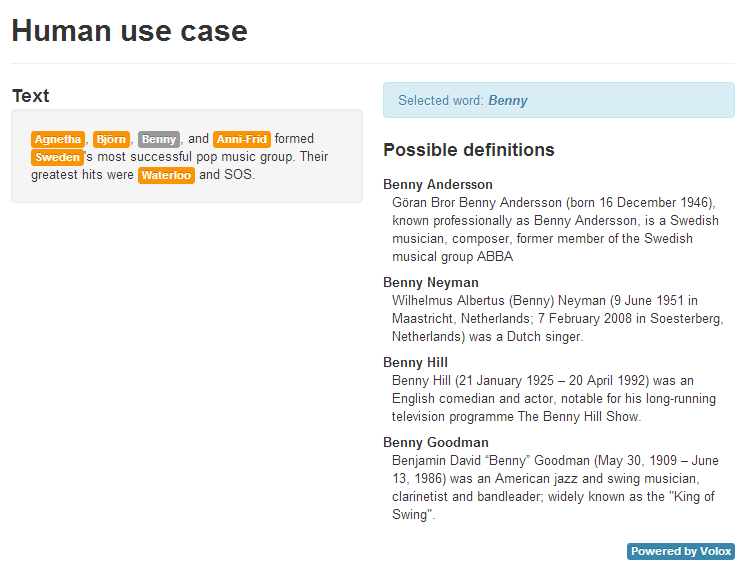
\includegraphics[width=0.8\columnwidth]{Human}
    \caption{Human use case Web interface.}
    \label{fig:human}
\end{figure}
The application (see \autoref{fig:human}) can be divided in two steps.
In the first step a text is
analyzed from the backend (YAGO2 or DBpedia) then, in the second step the
application asks to the user to disambiguate certain words that have not been
correctly understood.

In the second step for each ambiguous work the user have a list of possible
meanings to choose from. Once the user selected the correct word interpretation
it is saved into the browser.

Eventually when the user has disambiguated all the words he/she can send the
results back to the framework, where they are saved and stored for improving the
precision of the \ac{WSD} algorithm itself.





















\subsection{Hybrid}
In this scenario we have the human and the automatic computation blended together.
As explained in \ref{sec:cases:hybrid}, this use-case is implemented in two
parts: the face detection and the \ac{GWAP} logic.\\

\begin{figure}[htb]
    \centering
    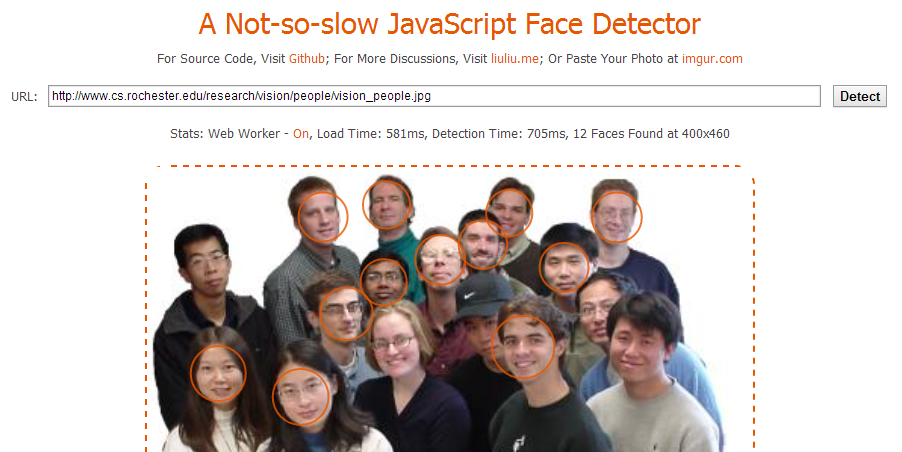
\includegraphics[width=0.75\columnwidth]{face-algo}
    \caption{Face detection algorithm demo.}
    \label{fig:face-algo}
\end{figure}

The face detection logic is implemented using an external library  by
\href{http://liuliu.me/}{Liu Liu} (see \autoref{fig:face-algo}). This library allow to detect face in an image
using the \js{} features presented in (like \code{Canvas} and \code{WebWorkers}).
The technique used to implement the algorithm will not be covered here but you
can find a detailed explanation here:
\url{http://liuliu.me/eyes/javascript-face-detection-explained/}.
The library\footnote{Source code: \url{https://github.com/liuliu/ccv/tree/unstable/js}}
can be used with or without WebWorkers to further increase the processing
speed\footnote{Demo available here: \url{http://liuliu.me/ccv/js/nss/}}.\\


The \ac{GWAP} follows the game logic presented in \ref{case:hybrid:gameplay} an
it has been implemented using the \ac{HTML}5 features.

Objective of the game is being able to identify the visage of the subject
portrayed in a photo. The provided algorithm for face detection may fail in this
task, by recognizing objects that are not the required ones (e.g. knees) or not
recognizing at all the face of a person. For this reason the game will be able
to perform two different tasks: identify faces that have not been recognized and
remove elements that have been marked improperly.

The game present the image with the bounding boxes of the faces that has been
identified by the first step to the player. The faces that have not been
recognized are the ones that the player needs to mark during the game by
clicking over them with the left mouse button and the area interested by the
click will be circumscribed in order to obtain the bounding box for the identified
face. 

Possible wrong bounding boxes will be removed by the player with the right mouse
button, in order to remove the false positives that may be identified by automatic
algorithms. Bounding boxes with high level confidence are kept into the image,
while bounding boxes with low level confidence values will be removed: it will
be a player duty to mark those faces by playing the game.

At the end of the execution we obtain a set of automatically detected faces plus
all the faces detected by the user. By intersecting this two set we could improve
the performance of our algorithm by adding the faces it was unable to find to
the training set.